\documentclass[tikz,border=6pt]{standalone}
\usepackage[T1]{fontenc}
\usetikzlibrary{positioning,arrows.meta}
\begin{document}
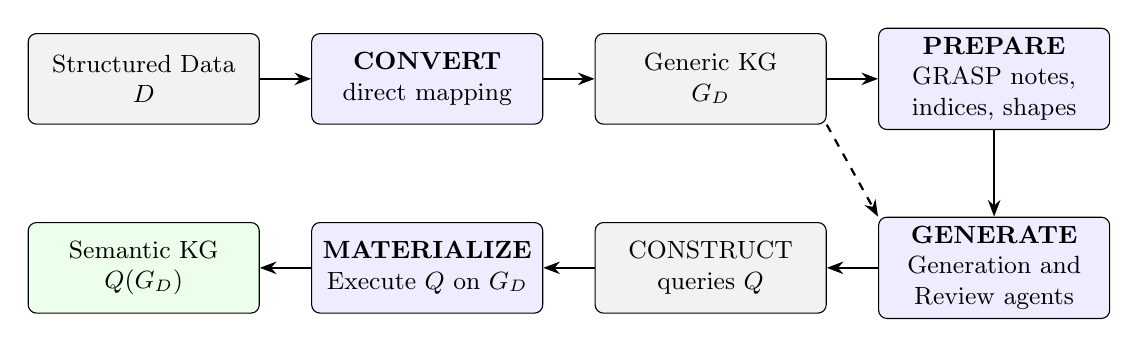
\begin{tikzpicture}[
  box/.style={draw, rounded corners=3pt, align=center, font=\small,
              minimum height=1.15cm, text width=2.7cm, fill=white},
  data/.style={box, fill=gray!10},
  stage/.style={box, fill=blue!7},
  final/.style={box, fill=green!8},
  arr/.style={-{Stealth[length=6pt]}, thick},
  lab/.style={font=\scriptsize, align=center}
]
\node[data] (d)   at (0,0)     {Structured Data\\$D$}; %(SQLite, CSV/TSV)
\node[stage] (c)   at (3.6,0)   {\textbf{CONVERT}\\direct mapping};
\node[data] (g)   at (7.2,0)   {Generic KG \\$G_D$}; %\\loaded in QLever
\node[stage] (s)   at (10.8,0)  {\textbf{PREPARE}\\GRASP notes,\\indices, shapes};
\node[stage] (q)   at (10.8,-2.4) {\textbf{GENERATE}\\Generation and\\Review agents};
\node[data] (qs)  at (7.2,-2.4)  {CONSTRUCT\\queries $Q$};
\node[stage] (m)   at (3.6,-2.4)  {\textbf{MATERIALIZE}\\Execute $Q$ on $G_D$};
\node[final] (o)   at (0,-2.4)    {Semantic KG\\$Q(G_D)$};
\draw[arr] (d) -- (c);
\draw[arr] (c) -- (g);
\draw[arr] (g) -- (s);
\draw[arr] (s) -- (q);
\draw[arr] (q) -- (qs);
\draw[arr] (qs) -- (m);
\draw[arr] (m) -- (o);
\draw[arr, dashed] (g.south east) -- (q.north west);
\end{tikzpicture}
\end{document}